\documentclass[11pt, a4paper]{article}

\usepackage{graphicx}
\usepackage[a4paper,top=3cm,bottom=2cm,left=2cm,right=2cm,marginparwidth=1.75cm]{geometry}
\usepackage[english]{babel}
\usepackage[utf8x]{inputenc}
\usepackage{subfig}
\usepackage{float}
\usepackage{amsmath}
\usepackage{amssymb}
\usepackage{mhchem}
\usepackage{hyperref}
\usepackage{tikz}
\usepackage{cancel}
\usepackage{bm}

\graphicspath{ {./images} }
\newcommand*{\qed}{\hfill\ensuremath{\quad\square}}%
\newcommand*{\rad}{\ensuremath{\,\text{rad}}}
\newcommand*{\R}{\ensuremath{\mathbb{R}}}
\newcommand*{\C}{\ensuremath{\mathbb{C}}}
\newcommand*{\m}{\text{m}}
\renewcommand*{\Re}{\operatorname{Re}}
\renewcommand*{\Im}{\operatorname{Im}}
\renewcommand*{\epsilon}{\varepsilon}
\renewcommand*{\phi}{\varphi}
\renewcommand*{\d}{\text{d}}


\DeclareRobustCommand{\uvec}[1]{{%
  \ifcat\relax\noexpand#1%
    % it should be a Greek letter
    \bm{\hat{#1}}%
  \else
    \ifcsname uvec#1\endcsname
      \csname uvec#1\endcsname
    \else
      \bm{\hat{\mathbf{#1}}}%
     \fi
   \fi
}}

\makeatletter
\renewcommand*\env@matrix[1][*\c@MaxMatrixCols c]{%
  \hskip -\arraycolsep
  \let\@ifnextchar\new@ifnextchar
  \array{#1}}
\makeatother

\newtheorem{theorem}{Theorem}
\numberwithin{equation}{section}
\numberwithin{figure}{section}

%------------------------------------------------
%Templates for images and figures
% \begin{figure}[h]
%   \centering
%   \subfloat[caption 1]{{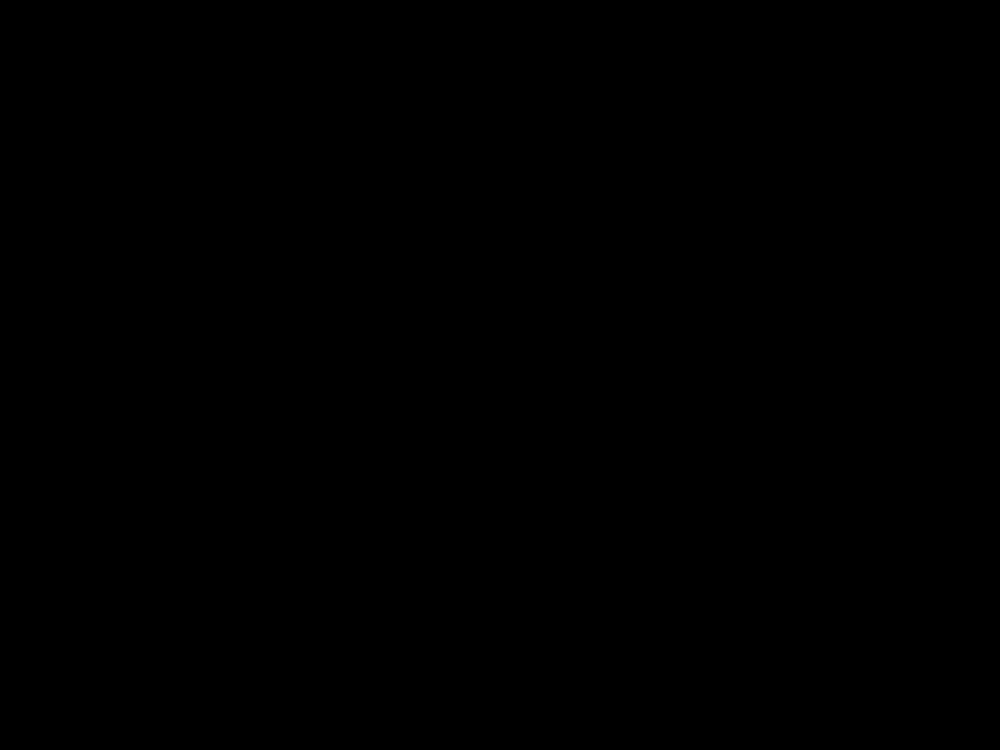
\includegraphics[width=30mm]{images/placeholder.png}}}%
%   \qquad
%   \subfloat[caption 2]{{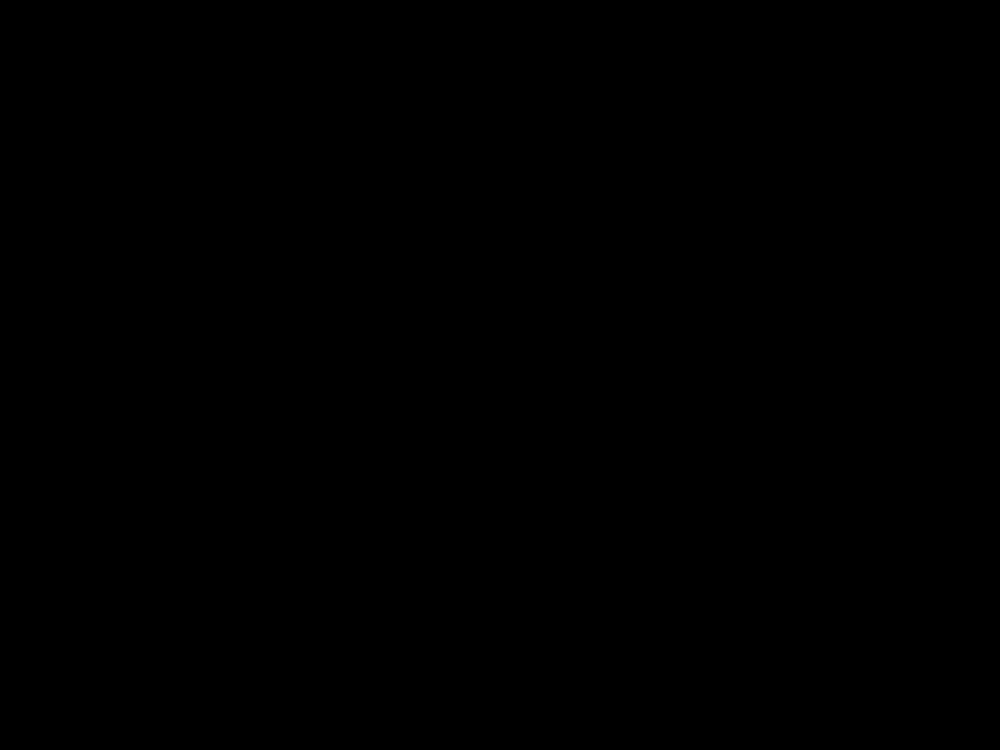
\includegraphics[width=30mm]{images/placeholder.png}}}%
%   \caption{Description}
% \end{figure}

% \begin{figure}[h]
%   \centerline{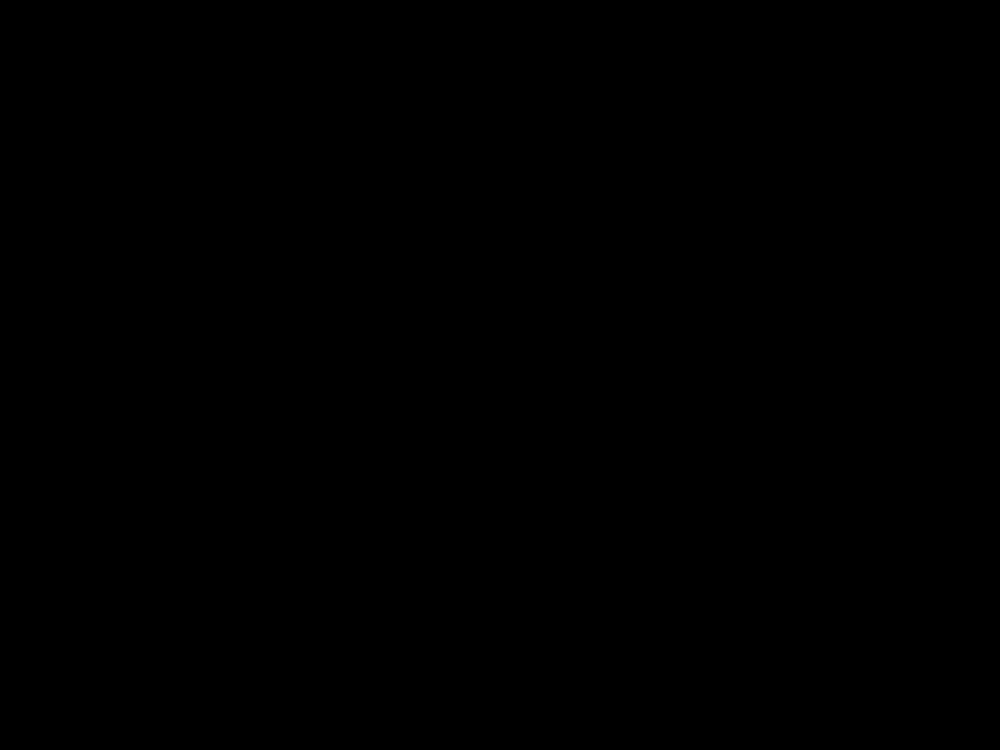
\includegraphics[width=50mm]{images/placeholder.png}}
%   \caption{Description}
% \end{figure}

%Template for a simple table 
%\begin{table}[h]
%   \caption{Description} %title of the table
%   \centering % centering table
%   \begin{tabular}{l rr} % creating three columns
%     \hline\hline %inserting double-line
%     & & \\ [0.5ex] % Insert half line vertical spacing
%     \hline % inserts single-line
%     & & \\ 
%     & & \\
%     & & \\
%     & & \\
%   \hline % inserts single-line
%   \end{tabular}
%   \label{tab:hresult}
% \end{table}
%-----------------------------------------------

\begin{document}
\setcounter{section}{3}
\section{Work and energy relations}


\subsection{Power and work of a force}
The instantaneuous power of a force $\vec{F}$ is defined as the scalar product of the force and the velocity of the particle or body:
\begin{equation}
  P = \vec{F}\cdot \vec{v}
\end{equation}
Note that instantaneuous power is a scalar rather then a vector. We can find the work done by a force by integrating the instantaneuous power at each moment in time with respect to time. Thus we find that:
\begin{equation}
  W = \int_{t_0}^{t_1} P\,\d t = \int_{t_0}^{t_1} \vec{F}\cdot\vec{v} \,\d t
\end{equation}
Since $\d\vec{r}$ can also be expressed as $\d\vec{r} = \vec{v}\d t$ we can express the work done by a force as the displacement of some particle or body over some path $\vec{r}$ as:
\begin{equation}
  W = \int_A^B \vec{F}\cdot\d\vec{r}
\end{equation}


\subsection{Work and energy relations}
The work done by some force $\vec{F}$ can be found by integrating along the path along which the force does work. A differential element of this path is given as $\d\vec{r}$:
\begin{equation}
  W = \int_A^B \vec{F}\cdot\d\vec{r} = m\int_A^B \vec{\ddot{r}}\cdot \d\vec{r}
\end{equation}
Integrating with respect to a vector is more work then it's worth, thus we look for a different way to express a differential element of the displacement vector:
\begin{equation}
  \d\vec{r} = \vec{\dot{r}}\d t
\end{equation}
This allows us to integrate with repsect to time, which is way easier. The expression for work then becomes:
\begin{equation}
  W = m\int_{t_0}^{t_1} \vec{\ddot{r}}\cdot \vec{\dot{r}} \d t = \left.\frac{1}{2}m(\vec{\dot{r}} \cdot \vec{\dot{r}})\right|_{t_0}^{t_1} = \frac{1}{2}m(\vec{v}_1^2 - \vec{v}_0^2)
\end{equation}
Kinetic energy is the amount of work required to change the velocity of a particle from resting velocity up untill the velocity $v$. This can be found by subsituting in $v_0 = 0\,\m/s$:
\begin{equation}
  T = \frac{1}{2}m|\vec{v}|^2 = \frac{1}{2}mv^2
\end{equation}
Because of this relation between work and kinetic energy we find that:
\begin{equation}
  W = \int_A^B \vec{F}\cdot \d\vec{r} = T_B - T_A = \Delta T
\end{equation}
Which means that the total work done by some force on a system will be the difference in kinetic energy, which in short is given as:
\begin{equation}
  W = \Delta T
\end{equation}
For a system of particles we define the total work of the system to be the summation of all the work done by all the internal and external forces acting on all the particles of the system. THis gives the following relation:
\begin{equation}
  W_i = \int_{A_i}^{B_i}\left( \vec{F}_i + \sum_{j=1}^{N}\vec{f}_{ij} \right) \cdot \d\vec{r}_i = \Delta T_i
\end{equation}
The kinetic energy of the individual particles is given as:
\begin{equation}
  T_i = \frac{1}{2}m_iv_i^2
\end{equation}
The total kinetic energy is then found by summing all of these individual kinetic energies together:
\begin{equation}
  T = \sum_{i=1}^{N} \frac{1}{2}m_iv_i^2
\end{equation}
Which we can subsitute back in our equation for work to find:
\begin{equation}
  W = \sum_{i=1}^{N} \int_{A_i}^{B_i}\left( \vec{F}_i + \sum_{j=1}^{N}\vec{f}_{ij} \right) \cdot \d\vec{r}_i = \sum_{i=1}^{N} T_i = \Delta T
\end{equation}


\subsection{Potential functions and conservative forces}
Of force is considered to be conservative if it conserves mechanical energy. The key to defining this mathematically is potential energy. We define the potential energy of a system to be some scalar function of the spatial coordinates: $V = V(x, y, z)$. If a force is conservative the total energy of the system should be constant. This means that the sum of potential and kinetic energy should be constant.
\begin{equation}
  T + V = c
\end{equation}
Where $c$ is some real constant. We can also express this in terms of difference in kinetic and potential energy. This will give the following relation:
\begin{equation}
  \Delta T + \Delta V = 0
\end{equation}
Since we know that difference in kinetic energy is the same as work we find that:
\begin{equation}
  W + \Delta V = 0
\end{equation}
We now consider an infinitesimal increment in both work and potential energy. This give the following expression:
\begin{equation}
  \d W + \d V = \vec{F}\cdot\d\vec{r} + \d V = 0
\end{equation}
Since we earlier defined the potential function $V$ to be a function of all $3$ spatial coordinates we need to use partial derrivatives to express a differential element of $V$:
\begin{align}
  \d V &= \frac{\partial V}{\partial x}\d x + \frac{\partial V}{\partial y}\d y + \frac{\partial V}{\partial z}\d z \\
  &=
  \begin{pmatrix}
    \frac{\partial V}{\partial x}\\
    \frac{\partial V}{\partial y}\\
    \frac{\partial V}{\partial z}
  \end{pmatrix}
  \cdot
  \begin{pmatrix}
    \d x\\
    \d y\\
    \d z
  \end{pmatrix}
  = \nabla V \cdot \d \vec{r}
\end{align}
If we subsitute this back in our equation we find that for a force to be conservative the following relation needs to hold:
\begin{equation}
  \vec{F} = -\nabla V
\end{equation}
This means that a force vector $\vec{F}$ is conservative if there exists some scalar function $V(x, y, z)$ whose gradient is the same as the negative of the force vector $\vec{F}$. 
\end{document}